\documentclass[11pt, oneside]{article} 
\usepackage{geometry}
\geometry{letterpaper} 
\usepackage{graphicx}
	
\usepackage{amssymb}
\usepackage{amsmath}
\usepackage{parskip}
\usepackage{color}
\usepackage{hyperref}

\graphicspath{{/Users/telliott_admin/Tex/png/}}
% \begin{center} 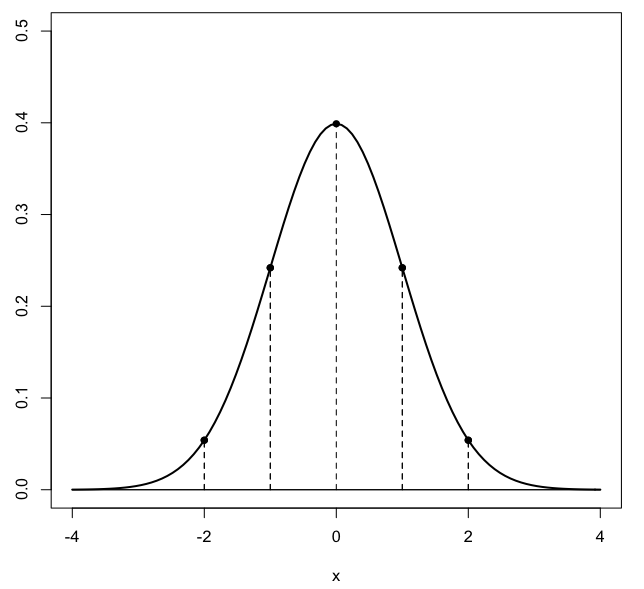
\includegraphics [scale=0.4] {gauss3.png} \end{center}

\title{Pi and 22/7}
\date{}

\begin{document}
\maketitle
\Large
An unusual wikipedia article within a collection of calculus topics contains a proof that $22/7 > \pi$.

\url{https://en.wikipedia.org/wiki/List_of_calculus_topics#Integral_calculus}

This isn't too hard to establish if you are calculating $\pi$ by one of the many known methods or simply remember
\[ \pi = 3.14159265 \dots \]

since $22/7 = 3\ 1/7$ and 
\[ 1/7 = 0.142857 \dots \]
repeating.

What's nice about this problem is there is a complicated-looking integral involved:
\[ \int_0^1 \frac{x^4(1-x)^4}{1 + x^2} \ dx \]

I have no idea where this expression came from yet, but it looks like we should be able to solve it.

\subsection*{proof}

The proof is the following:

First, the value of the integrand is zero at the bounds $[0,1]$ and very small but positive everywhere between (because of the powers $x^2$ and $x^4$).  

\begin{center} 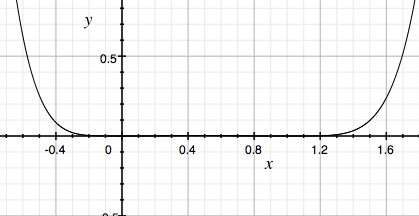
\includegraphics [scale=0.4] {pi_fraction.png} \end{center}

Since the integral is positive we can say that
\[ I > 0 \]

In fact, the integral can be solved, and it turns out to be equal to
\[ I = \frac{22}{7} - \pi \]
We obtain
\[ \frac{22}{7} - \pi  > 0 \]
which yields the promised inequality.
\[ \pi < \frac{22}{7} \]

\subsection*{algebra}

How to solve this?  Basically, what we do is multiply and divide to get a bunch of terms that we can integrate one by one.  The first step is to write the terms of
\[ (1-x)^4 =  1 - 4x + 6x^2 - 4x^3 + x^4 \]
from the binomial theorem, substituting $-x$ for $x$.

Now multiply by $x^4$ to obtain
\[ x^4 - 4x^5 + 6x^6 - 4x^7 + x^8 \]

The somewhat tricky part is the division by $1 + x^2$.  The first factor is $x^6$, since
\[ x^6 \cdot x^2 = x^8 \]
after subtracting that, we also need to subtract $x^6$ (obtained by multiplying by the $1$ in $1 + x^2$), leaving
\[ x^4 - 4x^5 + 5x^6 - 4x^7 \]

Next, we get a factor of $-4x^5 \cdot x^2 = -4x^7$, so then we also need to subtract $-4x^5$, leaving
\[ x^4 + 5x^6 \]

$5x^4 \cdot x^2 = 5x^6$, so then we need to subtract $5x^4$, leaving $-4x^4$
\[ -4x^4 \]

$-4x^2 \cdot x^2 = -4x^4$, so then we need to subtract $-4x^2$, leaving
\[ 4x^2 \]

$4 \cdot x^2 = 4x^2$, so then we need to subtract $4$, leaving 
\[ -4 \]
This last $-4$ is the remainder, still over $(1 + x^2)$.

Combining all these factors we have
\[ x^6 - 4x^5 + 5x^4 - 4x^2 + 4 - \frac{4}{1 + x^2} \]

Check by multiplying out by $1 + x^2$.  I get
\[ x^6 - 4x^5 + 5x^4 - 4x^2 + 4 + x^8 - 4x^7 + 5x^6 - 4x^4 + 4x^2 - 4 \]
\[ = x^8 - 4x^7 + 6x^6 - 4x^5 + x^4 \]
which seems correct.

\subsection*{integrating}
\[ \int_0^1 x^6 - 4x^5 + 5x^4 - 4x^2 + 4 - \frac{4}{1 + x^2} \]
The first five terms are easy:
\[ \frac{1}{7} - 4 \ \frac{1}{6} + 5 \ \frac{1}{5} - 4 \ \frac{1}{3} + 4 \]
\[ = \frac{1}{7} - \frac{2}{3} + 1 - \frac{4}{3} + 4 \]
\[ = 3 \ \frac{1}{7} = \frac{22}{7}  \]
The last term is
\[ \int_0^1 - \frac{4}{1 + x^2} = -4 \tan^{-1} x \ \bigg |_0^1 = -4 \cdot \frac{\pi}{4} = - \pi \]
Thus, finally we obtain
\[  \frac{22}{7} - \pi \]
as promised.


\end{document}